\documentclass[a4paper]{report}
% Some basic packages
\usepackage[utf8]{inputenc}
\usepackage[T1]{fontenc}
\usepackage{textcomp}
\usepackage[english]{babel}
\usepackage{url}
\usepackage{graphicx}
\usepackage{float}
\usepackage{booktabs}
\usepackage{enumitem}

\pdfminorversion=7

% Don't indent paragraphs, leave some space between them
\usepackage{parskip}

% Hide page number when page is empty
\usepackage{emptypage}
\usepackage{subcaption}
\usepackage{multicol}
\usepackage{xcolor}

% Other font I sometimes use.
% \usepackage{cmbright}

% Math stuff
\usepackage{amsmath, amsfonts, mathtools, amsthm, amssymb}
% Fancy script capitals
\usepackage{mathrsfs}
\usepackage{cancel}
% Bold math
\usepackage{bm}
% Some shortcuts
\newcommand\N{\ensuremath{\mathbb{N}}}
\newcommand\R{\ensuremath{\mathbb{R}}}
\newcommand\Z{\ensuremath{\mathbb{Z}}}
\renewcommand\O{\ensuremath{\emptyset}}
\newcommand\Q{\ensuremath{\mathbb{Q}}}
\newcommand\C{\ensuremath{\mathbb{C}}}
\renewcommand\L{\ensuremath{\mathcal{L}}}

% Package for Petri Net drawing
\usepackage[version=0.96]{pgf}
\usepackage{tikz}
\usetikzlibrary{arrows,shapes,automata,petri}
\usepackage{tikzit}
\input{petri_nets_style.tikzstyles}

% Easily typeset systems of equations (French package)
\usepackage{systeme}

% Put x \to \infty below \lim
\let\svlim\lim\def\lim{\svlim\limits}

%Make implies and impliedby shorter
\let\implies\Rightarrow
\let\impliedby\Leftarrow
\let\iff\Leftrightarrow
\let\epsilon\varepsilon

% Add \contra symbol to denote contradiction
\usepackage{stmaryrd} % for \lightning
\newcommand\contra{\scalebox{1.5}{$\lightning$}}

% \let\phi\varphi

% Command for short corrections
% Usage: 1+1=\correct{3}{2}

\definecolor{correct}{HTML}{009900}
\newcommand\correct[2]{\ensuremath{\:}{\color{red}{#1}}\ensuremath{\to }{\color{correct}{#2}}\ensuremath{\:}}
\newcommand\green[1]{{\color{correct}{#1}}}

% horizontal rule
\newcommand\hr{
    \noindent\rule[0.5ex]{\linewidth}{0.5pt}
}

% hide parts
\newcommand\hide[1]{}

% si unitx
\usepackage{siunitx}
\sisetup{locale = FR}

% Environments
\makeatother
% For box around Definition, Theorem, \ldots
\usepackage{mdframed}
\mdfsetup{skipabove=1em,skipbelow=0em}
\theoremstyle{definition}
\newmdtheoremenv[nobreak=true]{definitie}{Definitie}
\newmdtheoremenv[nobreak=true]{eigenschap}{Eigenschap}
\newmdtheoremenv[nobreak=true]{gevolg}{Gevolg}
\newmdtheoremenv[nobreak=true]{lemma}{Lemma}
\newmdtheoremenv[nobreak=true]{propositie}{Propositie}
\newmdtheoremenv[nobreak=true]{stelling}{Stelling}
\newmdtheoremenv[nobreak=true]{wet}{Wet}
\newmdtheoremenv[nobreak=true]{postulaat}{Postulaat}
\newmdtheoremenv{conclusie}{Conclusie}
\newmdtheoremenv{toemaatje}{Toemaatje}
\newmdtheoremenv{vermoeden}{Vermoeden}
\newtheorem*{herhaling}{Herhaling}
\newtheorem*{intermezzo}{Intermezzo}
\newtheorem*{notatie}{Notatie}
\newtheorem*{observatie}{Observatie}
\newtheorem*{exe}{Exercise}
\newtheorem*{opmerking}{Opmerking}
\newtheorem*{praktisch}{Praktisch}
\newtheorem*{probleem}{Probleem}
\newtheorem*{terminologie}{Terminologie}
\newtheorem*{toepassing}{Toepassing}
\newtheorem*{uovt}{UOVT}
\newtheorem*{vb}{Voorbeeld}
\newtheorem*{vraag}{Vraag}

\newmdtheoremenv[nobreak=true]{definition}{Definition}
\newtheorem*{eg}{Example}
\newtheorem*{notation}{Notation}
\newtheorem*{previouslyseen}{As previously seen}
\newtheorem*{remark}{Remark}
\newtheorem*{note}{Note}
\newtheorem*{problem}{Problem}
\newtheorem*{observe}{Observe}
\newtheorem*{property}{Property}
\newtheorem*{intuition}{Intuition}
\newmdtheoremenv[nobreak=true]{prop}{Proposition}
\newmdtheoremenv[nobreak=true]{theorem}{Theorem}
\newmdtheoremenv[nobreak=true]{corollary}{Corollary}

% End example and intermezzo environments with a small diamond (just like proof
% environments end with a small square)
\usepackage{etoolbox}
\AtEndEnvironment{vb}{\null\hfill$\diamond$}%
\AtEndEnvironment{intermezzo}{\null\hfill$\diamond$}%
% \AtEndEnvironment{opmerking}{\null\hfill$\diamond$}%

% Fix some spacing
% http://tex.stackexchange.com/questions/22119/how-can-i-change-the-spacing-before-theorems-with-amsthm
\makeatletter
\def\thm@space@setup{%
  \thm@preskip=\parskip \thm@postskip=0pt
}


% Exercise 
% Usage:
% \exercise{5}
% \subexercise{1}
% \subexercise{2}
% \subexercise{3}
% gives
% Exercise 5
%   Exercise 5.1
%   Exercise 5.2
%   Exercise 5.3
\newcommand{\exercise}[1]{%
    \def\@exercise{#1}%
    \subsection*{Exercise #1}
}

\newcommand{\subexercise}[1]{%
    \subsubsection*{Exercise \@exercise.#1}
}


% \lecture starts a new lecture (les in dutch)
%
% Usage:
% \lecture{1}{di 12 feb 2019 16:00}{Inleiding}
%
% This adds a section heading with the number / title of the lecture and a
% margin paragraph with the date.

% I use \dateparts here to hide the year (2019). This way, I can easily parse
% the date of each lecture unambiguously while still having a human-friendly
% short format printed to the pdf.

\usepackage{xifthen}
\def\testdateparts#1{\dateparts#1\relax}
\def\dateparts#1 #2 #3 #4 #5\relax{
    \marginpar{\small\textsf{\mbox{#1 #2 #3 #5}}}
}

\def\@lecture{}%
\newcommand{\lecture}[3]{
    \ifthenelse{\isempty{#3}}{%
        \def\@lecture{Lecture #1}%
    }{%
        \def\@lecture{Lecture #1: #3}%
    }%
    \subsection*{\@lecture}
    \marginpar{\small\textsf{\mbox{#2}}}
}



% These are the fancy headers
\usepackage{fancyhdr}
\pagestyle{fancy}

% LE: left even
% RO: right odd
% CE, CO: center even, center odd
% My name for when I print my lecture notes to use for an open book exam.
% \fancyhead[LE,RO]{Gilles Castel}

\fancyhead[RO,LE]{\@lecture} % Right odd,  Left even
\fancyhead[RE,LO]{}          % Right even, Left odd

\fancyfoot[RO,LE]{\thepage}  % Right odd,  Left even
\fancyfoot[RE,LO]{}          % Right even, Left odd
\fancyfoot[C]{\leftmark}     % Center

\makeatother




% Todonotes and inline notes in fancy boxes
\usepackage{todonotes}
\usepackage{tcolorbox}

% Make boxes breakable
\tcbuselibrary{breakable}

% Verbetering is correction in Dutch
% Usage: 
% \begin{verbetering}
%     Lorem ipsum dolor sit amet, consetetur sadipscing elitr, sed diam nonumy eirmod
%     tempor invidunt ut labore et dolore magna aliquyam erat, sed diam voluptua. At
%     vero eos et accusam et justo duo dolores et ea rebum. Stet clita kasd gubergren,
%     no sea takimata sanctus est Lorem ipsum dolor sit amet.
% \end{verbetering}
\newenvironment{verbetering}{\begin{tcolorbox}[
    arc=0mm,
    colback=white,
    colframe=green!60!black,
    title=Opmerking,
    fonttitle=\sffamily,
    breakable
]}{\end{tcolorbox}}

% Noot is note in Dutch. Same as 'verbetering' but color of box is different
\newenvironment{noot}[1]{\begin{tcolorbox}[
    arc=0mm,
    colback=white,
    colframe=white!60!black,
    title=#1,
    fonttitle=\sffamily,
    breakable
]}{\end{tcolorbox}}




% Figure support as explained in my blog post.
\usepackage{import}
\usepackage{xifthen}
\usepackage{pdfpages}
\usepackage{transparent}
\newcommand{\incfig}[1]{%
    \def\svgwidth{\columnwidth}
    \import{./figures/}{#1.pdf_tex}
}

% Fix some stuff
% %http://tex.stackexchange.com/questions/76273/multiple-pdfs-with-page-group-included-in-a-single-page-warning
\pdfsuppresswarningpagegroup=1


% My name
\author{Bruno M. Pacheco}

 
\begin{document}

\title{Relatório 7}
\author{Bruno M. Pacheco\\
DAS 5142 - Sistemas Dinâmicos}
 
\maketitle

\exercise{E1}

\subexercise{a)}

Podemos modelar os sistema proposto através da seguinte equação:
\begin{align*}
    & \dot{h}(t) = \frac{500}{\pi\left( Dh - h^2 \right) }u(t) - \frac{A_2\sqrt{2gh} }{\pi\left( Dh - h^2 \right) } \\
    & 0\le h(t)\le 100
.\end{align*}

Linearizando esse sistema em torno de um ponto de operação $\overline{h}$, temos \[
h(t) = \overline{h} + \Delta h(t)
,\] ou seja, reduzimos o sistema à sua variação linear $\Delta h(t)$ em torno do ponto de equilíbrio. Encontramos $\overline{u}$ sabendo que, para um dado ponto de operação $\overline{h}$, é verdade que \[
\frac{d h(t)}{dt}\Bigr|_{(\overline{h},\overline{u})} = 0
.\] Para a dinâmica do modelo, vemos que
\begin{align*}
    \dot{h}(t) &= \Delta \dot{h}(t) = \frac{\delta \Delta \dot{h}}{\delta h}\Bigr|_{(\overline{h},\overline{u})}\Delta h(t) + \frac{\delta \Delta \dot{h}}{\delta u}\Bigr|_{(\overline{h},\overline{u})}\Delta u(t) \\
    a &= \frac{\delta \Delta \dot{h}}{\delta h}\Bigr|_{(\overline{h},\overline{u})} = \frac{-A_2g}{\pi\left( D\overline{h}- \overline{h}^2 \right)\sqrt{2g\overline{h}}}\\
    b &= \frac{\delta \Delta \dot{h}}{\delta u}\Bigr|_{(\overline{h},\overline{u})} = \frac{500}{\pi\left( D \overline{h}- \overline{h}^2 \right) } \\
.\end{align*}

Assim, vemos que o sistema resultante pode ser modelado no domínio da frequência complexa por \[
    \frac{\Delta H(s)}{U(s)} = \frac{b}{s-a} = \frac{k}{\tau s + 1}
,\] onde $k=\frac{-b}{a}$ e $\tau = \frac{-1}{a}$.

Essa linearização foi implementada no \emph{Simulink} conforme pode ser visto na figura \ref{fig:figures-lab7_simulink_MA-png}.

\begin{figure}[H]
    \centering
    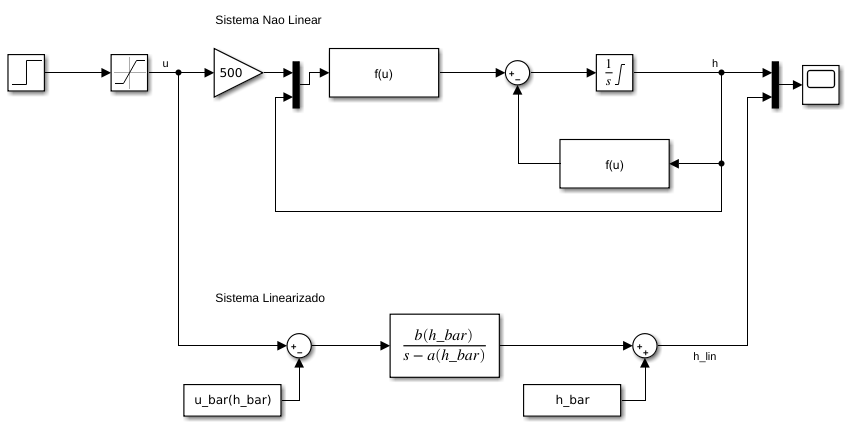
\includegraphics[width=0.8\textwidth]{figures/lab7_simulink_MA.png}
    \caption{Implementação do sistema linearizado e não linear no \emph{Simulink}.}
    \label{fig:figures-lab7_simulink_MA-png}
\end{figure}

Para o projeto do controlador nos pontos de operação, utilizou-se a ferramenta \emph{rltool} do Matlab. Assim, chegou-se aos valores do controlador conforme a tabela \ref{tab:ganhos-PI}.

\begin{table}[H]
    \centering
    \caption{Ganhos dos controladores PI projetados para os pontos de operação $\overline{h}$.}
    \label{tab:ganhos-PI}
    \begin{tabular}{c | c | c}
	$\overline{h}$ & $K_c$ & $K_i$ \\
	\hline 
	10 & 2,2129 & 0,2154 \\
	50 & 6,7742 & 0,1770 \\
	90 & 2,0389 & 0,1887
    \end{tabular}
\end{table}

O controlador com esses ganhos foi implementado no \emph{simulink}. A implementação do sistema em malha fechada pode ser observada na figura \ref{fig:figures-lab7_simulink_MF-png}. Nota-se que ambos os sistemas original e linearizado foram implementados.

\begin{figure}[H]
    \centering
    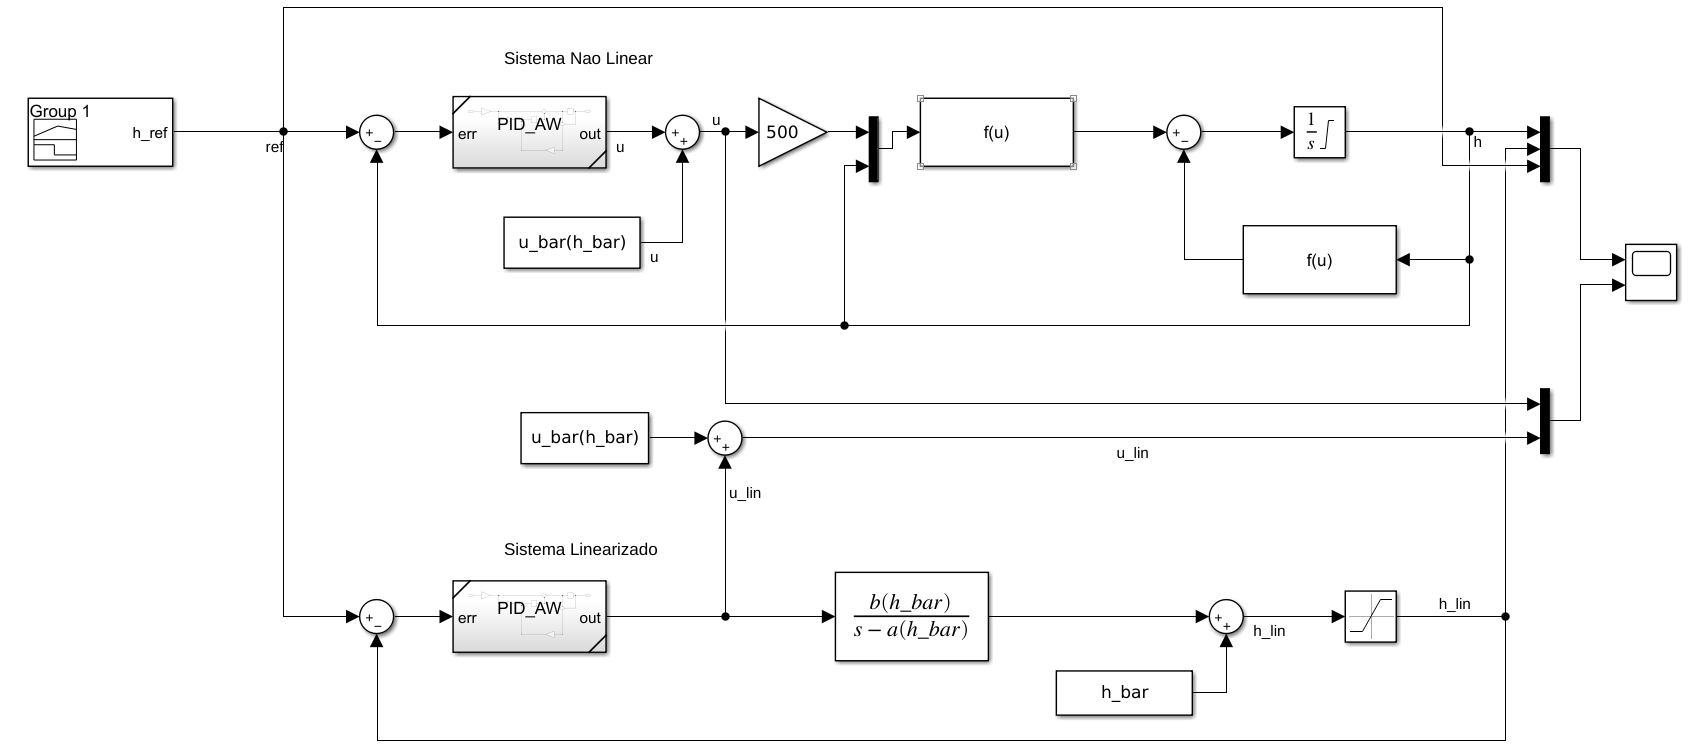
\includegraphics[width=0.8\textwidth]{figures/lab7_simulink_MF.png}
    \caption{Implementação do sistema em malha fechada com o controlador PI.}
    \label{fig:figures-lab7_simulink_MF-png}
\end{figure}

Simulou-se a resposta de ambos os sistemas implementados à degraus entre os pontos de operação. O resultado pode ser observado na figura \ref{fig:figures-lab4_1_resposta_simulink}.

\begin{figure}[H]
    \centering
    \begin{subfigure}{0.32\textwidth}
	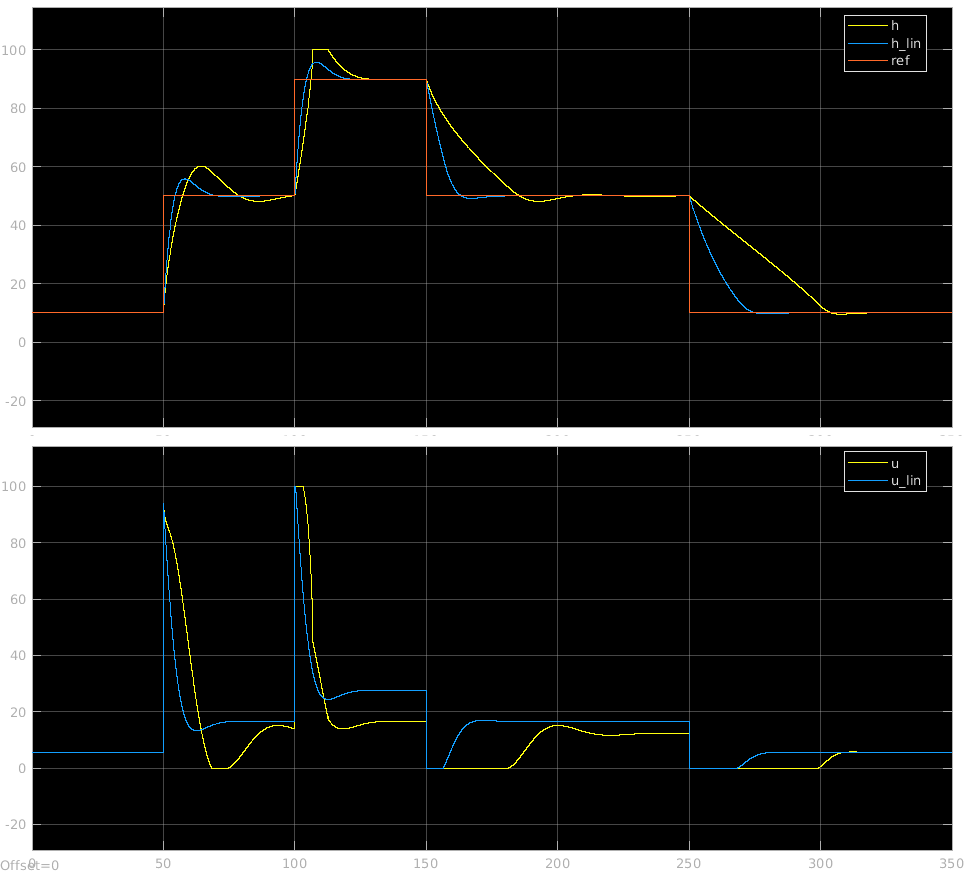
\includegraphics[width=\textwidth]{figures/lab7_PI_10.png}
	\caption{$\overline{h} = 10$.}
    \end{subfigure}
    \begin{subfigure}{0.32\textwidth}
	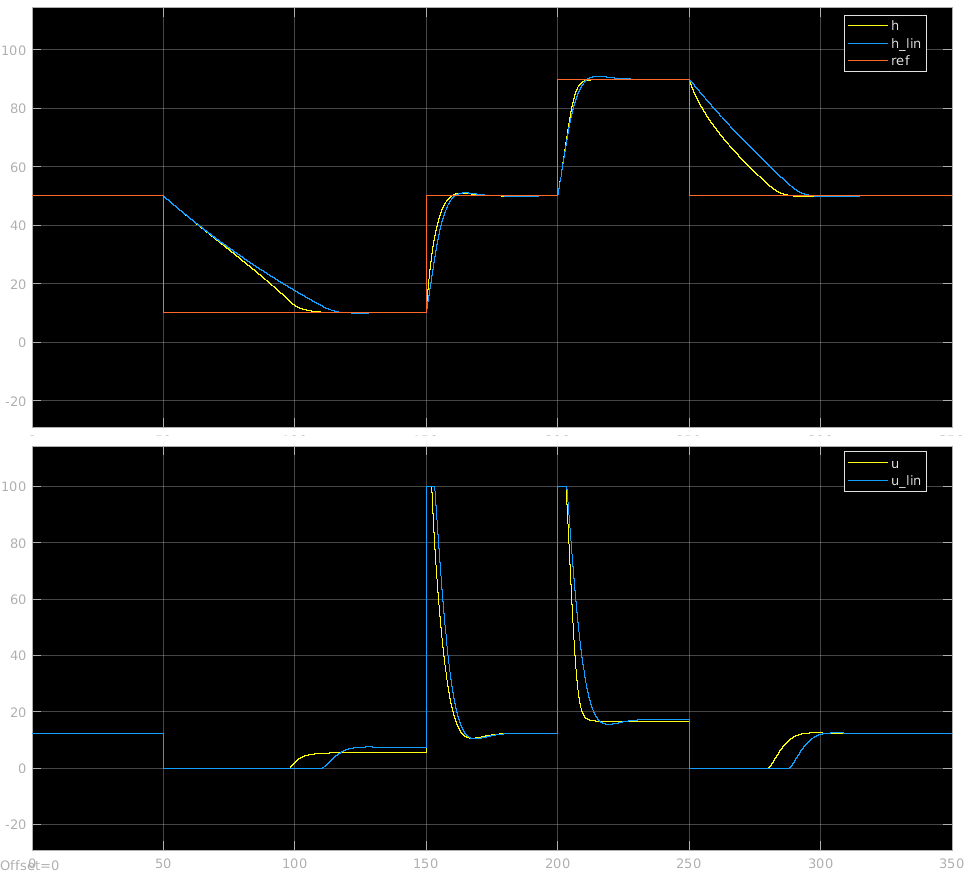
\includegraphics[width=\textwidth]{figures/lab7_PI_50.png}
	\caption{$\overline{h} = 50$.}
    \end{subfigure}
    \begin{subfigure}{0.32\textwidth}
	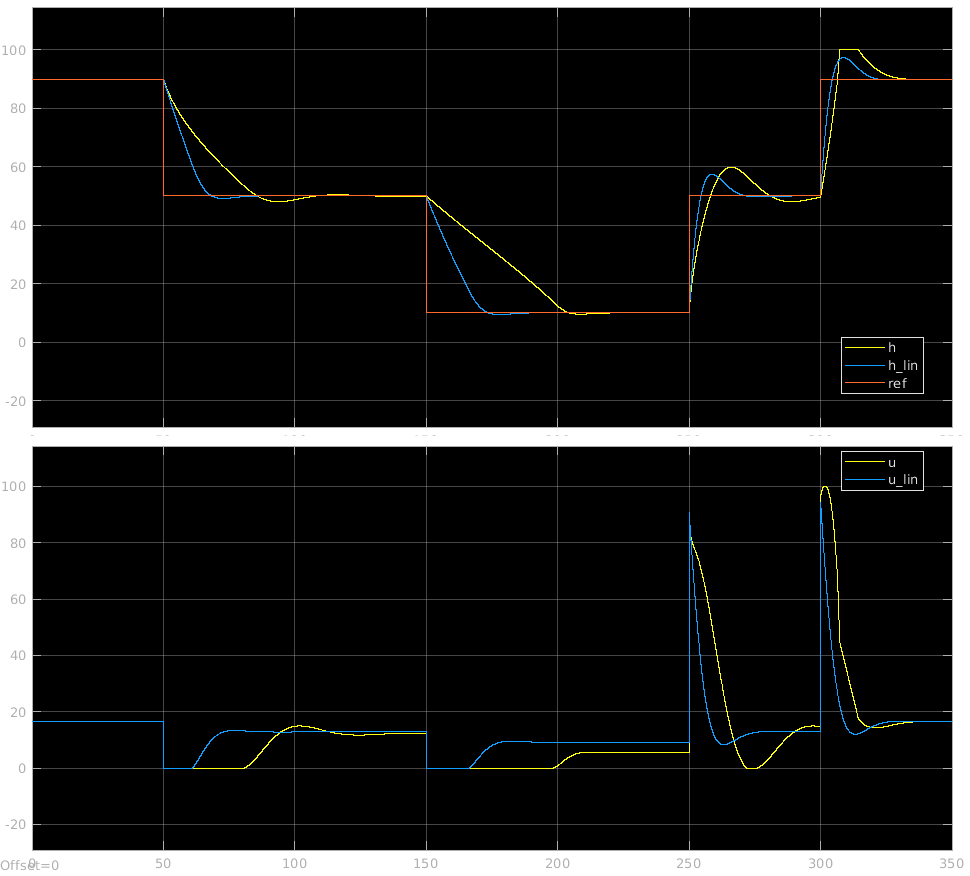
\includegraphics[width=\textwidth]{figures/lab7_PI_90.png}
	\caption{$\overline{h} = 90$.}
    \end{subfigure}
    \caption{Resposta dos sistemas em malha fechada à troca de ponto de operação.}
    \label{fig:figures-lab4_1_resposta_simulink}
\end{figure}

\subexercise{b)}

A partir do equacionamento não linear do sistema, desejamos encontrar um FLC. Assim, temos
\begin{align*}
    & \dot{h}(t) = \frac{500u(t) - A_2\sqrt{2gh} }{\pi\left( Dh - h^2 \right) } = v(t)\\
,\end{align*}
onde $v(t)$ é a saída do controlador linear desejado. Assim, podemos determinar a nova entrada para a planta como \[
    u(t) = \frac{v(t)\pi\left( Dh - h^2 \right) + A_2\sqrt{2gh} }{500}
,\] o que resulta em um novo sistema \[
\dot{h}(t) = v(t) + \frac{A_2\sqrt{2gh(t)} - A_2\sqrt{2gh(t)}  }{\pi\left( Dh(t) h^2(t) \right) } = v(t)
,\] considerando que a identificação de $A_2$ é perfeita.

Para a implementação do controle, podemos entender $u(t)$ como \[
    u(t) = f(h) + g(h)v(t)
,\] onde
\begin{align*}
    f(h) &= \frac{A_2\sqrt{2gh} }{500} \\
    g(h) &= \frac{\pi\left( Dh - h^2 \right) }{500}
.\end{align*}
Além disso, para garantirmos que o acionamento se mantém nos níveis aceitos pelo sistema propaga-se a saturação para $v(t)$, de forma que \[
    \frac{-f(h)}{g(h)} < v(t) < \frac{100-f(h)}{g(h)}
.\] 

A partir disso, implementou-se o controle linearizante conforme visível na figura \ref{fig:figures-lab7_FLC-png}. Destaca-se o uso de valores aproximados para os limites de saturação para evitar erros numéricos.

\begin{figure}[H]
    \centering
    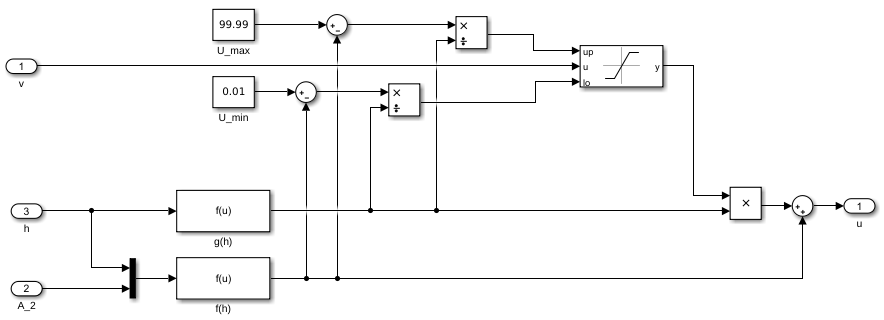
\includegraphics[width=0.8\textwidth]{figures/lab7_FLC.png}
    \caption{Controle linearizante implementado no Simulink.}
    \label{fig:figures-lab7_FLC-png}
\end{figure}

Para o controle, implementou-se a lei de controle \[
v(t) = \dot{h}_r + K_0e(t)
,\] que foi implementada junto à planta conforme visível na figura \ref{fig:figures-lab7_FLC_simulink-png}.

\begin{figure}[H]
    \centering
    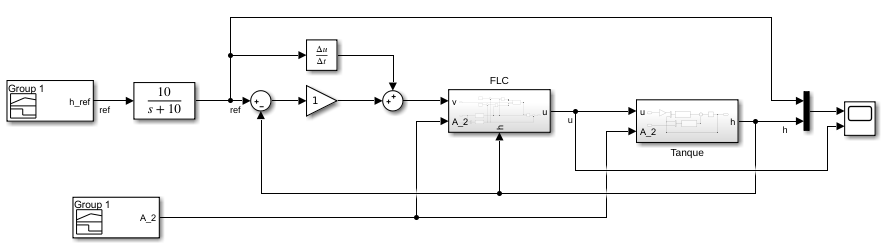
\includegraphics[width=0.8\textwidth]{figures/lab7_FLC_simulink.png}
    \caption{Implementação do sistema em malha fechada com controlador.}
    \label{fig:figures-lab7_FLC_simulink-png}
\end{figure}

Assim, a resposta do sistema pode ser observada na figura \ref{fig:figures-lab7_b_result-png}. Um ajuste fino do ganho $K_0$ foi realizado mas, pelo baixo impacto, optou-se por mantê-lo unitário. O aprimoramento da resposta é claro quando comparado à figura \ref{fig:figures-lab4_1_resposta_simulink}, com um tempo de acomodação significativamente maior e sem nenhum sobressinal.

\begin{figure}[H]
    \centering
    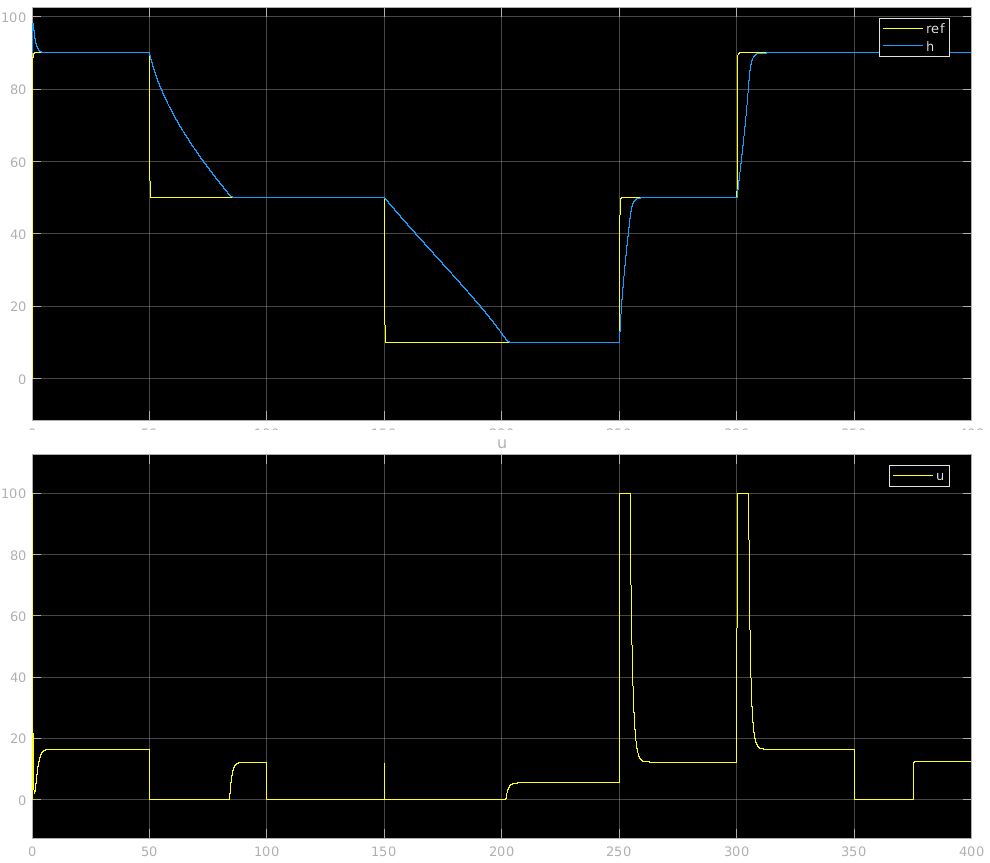
\includegraphics[width=0.8\textwidth]{figures/lab7_b_result.png}
    \caption{Resposta do sistema à variação na referência.}
    \label{fig:figures-lab7_b_result-png}
\end{figure}

\subexercise{c)}

Para analisar a robustez do sistema, fixamos o parâmetro $A_2$ do ponto de vista do controlador linearizante e variamos o valor real desse parâmetro na planta. A resposta do sistema nesse cenário pode ser observada na figura \ref{fig:figures-lab7_c_resposta-png}.

\begin{figure}[H]
    \centering
    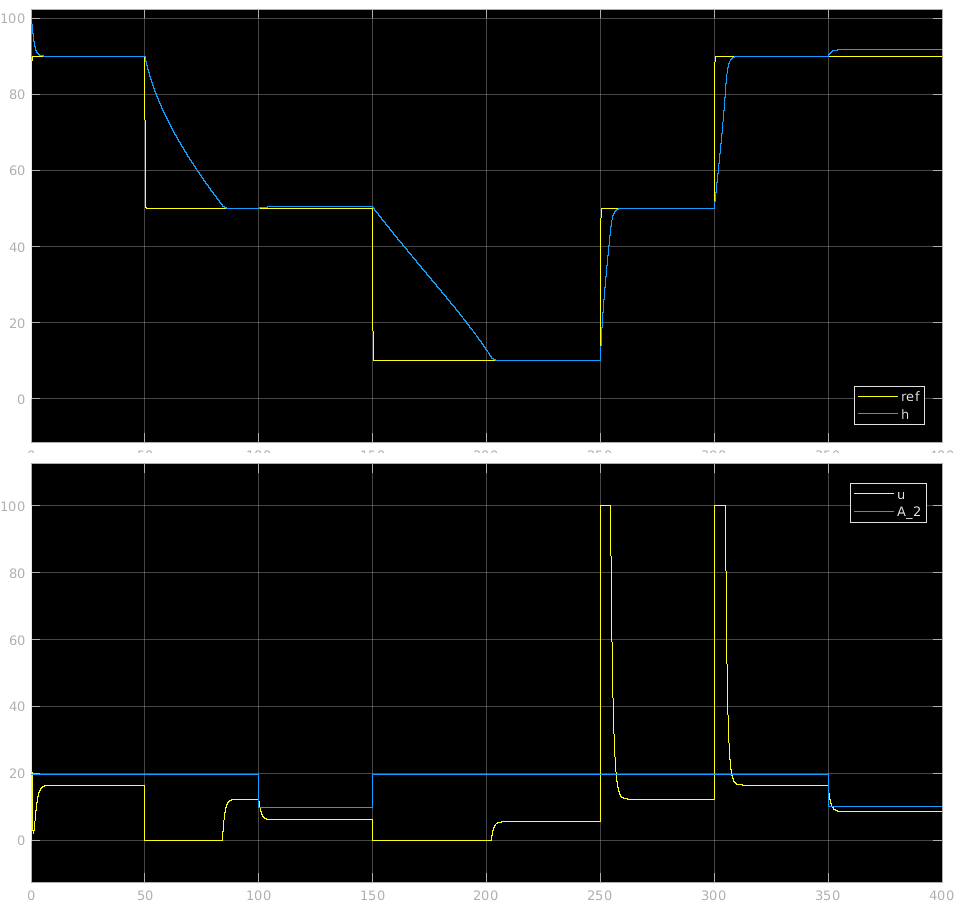
\includegraphics[width=0.8\textwidth]{figures/lab7_c_resposta.png}
    \caption{Resposta do sistema com variação do parâmetro $A_2$ da planta.}
    \label{fig:figures-lab7_c_resposta-png}
\end{figure}

Vê-se que com uma variação do parâmetro $A_2$ a erro não é mais anulado, ou seja, já não mais se atinge a referência em regime permanente.

\subexercise{d)}

Além de incluir uma ação integral no controlador, podemos atuar estimando $A_2$ a partir do modelo do sistema, ou seja, sabendo o comportamento do sistema, podemos, a partir do conhecimento da entrada e da saída, estimar o parâmetro desconhecido. Dessa forma, podemos estimar \[
    \hat{A_2} = K_2 \left( h(t) - \hat{h}(t) \right) 
,\] onde $\hat{h}(t)$ é a nossa estimativa do estado do sistema a partir de um observador.

A implementação do observador pode ser observada na figura \ref{fig:lab7_obs-png}.

\begin{figure}[H]
    \centering
    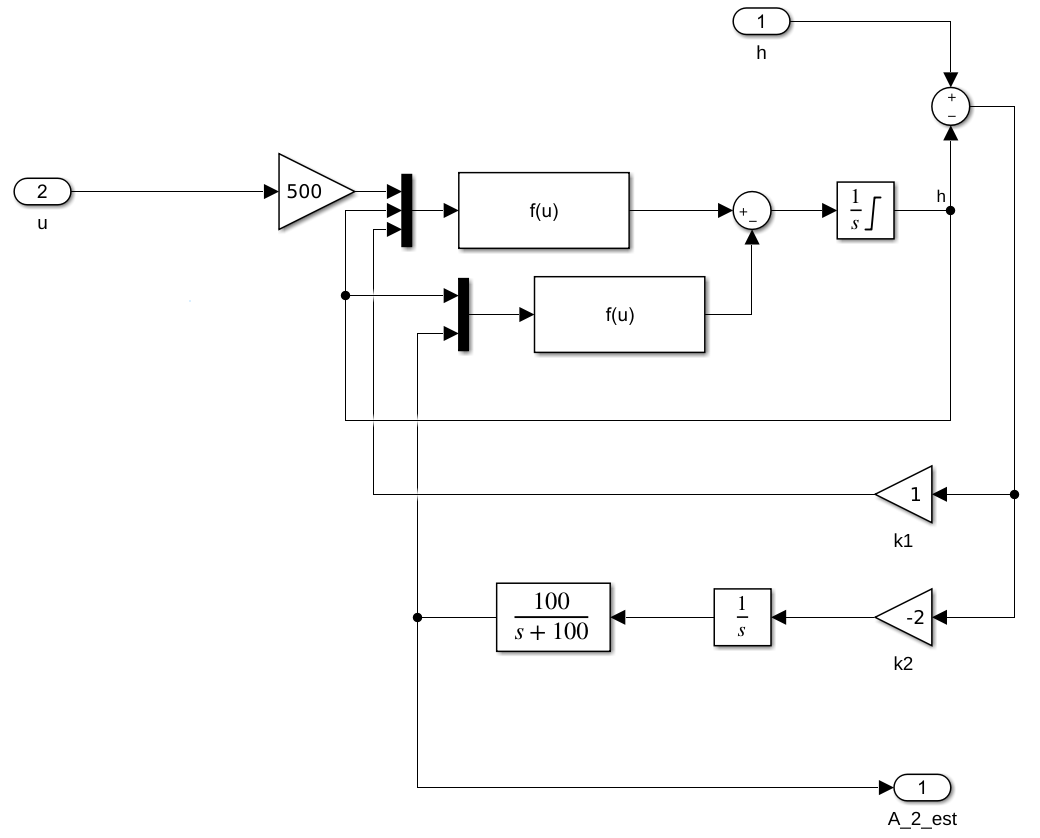
\includegraphics[width=0.8\textwidth]{figures/lab7_obs.png}
    \caption{Implementação do observador.}
    \label{fig:figures-lab7_obs-png}
\end{figure}

A reposta do sistema com o observador pode ser observada na figura \ref{asdf}. Podemos notar que o sistema corrige a sua estimativa do parâmetro $A_2$ com erro 0 em regime permanente, o que resulta novamente em uma anulação no erro em regime permanente da saída controlada.

\begin{figure}[H]
    \centering
    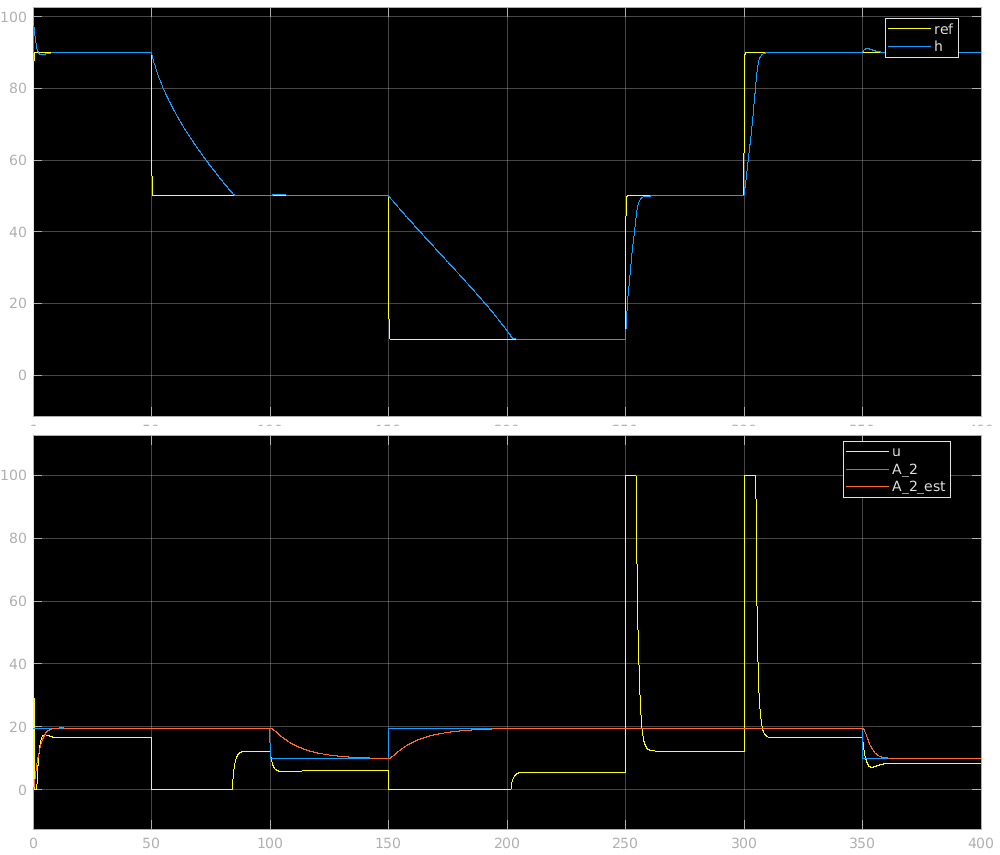
\includegraphics[width=0.8\textwidth]{figures/lab7_obs_plot.png}
    \caption{Resposta do sistema com observador à variação do parâmetro $A_2$.}
    \label{asdf}
\end{figure}

\end{document}
